% This is the University of Chicago Graham School Master of Science in Analytics
% template. Much of it is based on the Reed College LaTeX thesis template.
% Most of the work for the Reec College template was done by Sam Noble (SN),
% Later comments etc. by Ben Salzberg (BTS).
% Additional restructuring and APA support by Jess Youngberg (JY).
% Justin M. Shea (JMS) built on their good open source work.
% Your comments and suggestions are more than welcome:
% please email, them to justinshea@uchicago.edu.
%
% Any line that starts with a percent symbol is a comment.
% They won't show up in the document, and are useful for notes
% to yourself and explaining commands.
% Commenting also removes a line from the document;
% very handy for troubleshooting problems. -BTS
%%
%% Preamble
%%
% \documentclass{<something>} must begin each LaTeX document
% Added by JMS
\documentclass[12pt,oneside]{chicagocapstone}
% END of JMS add
% Packages are extensions to the basic LaTeX functions. Whatever you
% want to typeset, there is probably a package out there for it.
% Check out CTAN to see: http://www.ctan.org/
%%
\usepackage{graphicx,latexsym}
\usepackage{amsmath}
\usepackage{amssymb,amsthm}
\usepackage{longtable,booktabs,setspace}
\usepackage[hyphens]{url}
% Added by CII
\usepackage{hyperref}
\usepackage{lmodern}
\usepackage{float}
\floatplacement{figure}{H}
% End of CII addition
\usepackage{rotating}


% Added by CII (Thanks, Hadley!)
% Use ref for internal links
\renewcommand{\hyperref}[2][???]{\autoref{#1}}
\def\chapterautorefname{Chapter}
\def\sectionautorefname{Section}
\def\subsectionautorefname{Subsection}
% End of CII addition

% Added by CII
\usepackage{caption}
\captionsetup{width=5in}
% End of CII addition

% Added by JMS
\usepackage{mathptmx} % Times New Roman fonts
% End of add by JMS

% Syntax highlighting #22
  \usepackage{color}
  \usepackage{fancyvrb}
  \newcommand{\VerbBar}{|}
  \newcommand{\VERB}{\Verb[commandchars=\\\{\}]}
  \DefineVerbatimEnvironment{Highlighting}{Verbatim}{commandchars=\\\{\}}
  % Add ',fontsize=\small' for more characters per line
  \usepackage{framed}
  \definecolor{shadecolor}{RGB}{248,248,248}
  \newenvironment{Shaded}{\begin{snugshade}}{\end{snugshade}}
  \newcommand{\KeywordTok}[1]{\textcolor[rgb]{0.13,0.29,0.53}{\textbf{#1}}}
  \newcommand{\DataTypeTok}[1]{\textcolor[rgb]{0.13,0.29,0.53}{#1}}
  \newcommand{\DecValTok}[1]{\textcolor[rgb]{0.00,0.00,0.81}{#1}}
  \newcommand{\BaseNTok}[1]{\textcolor[rgb]{0.00,0.00,0.81}{#1}}
  \newcommand{\FloatTok}[1]{\textcolor[rgb]{0.00,0.00,0.81}{#1}}
  \newcommand{\ConstantTok}[1]{\textcolor[rgb]{0.00,0.00,0.00}{#1}}
  \newcommand{\CharTok}[1]{\textcolor[rgb]{0.31,0.60,0.02}{#1}}
  \newcommand{\SpecialCharTok}[1]{\textcolor[rgb]{0.00,0.00,0.00}{#1}}
  \newcommand{\StringTok}[1]{\textcolor[rgb]{0.31,0.60,0.02}{#1}}
  \newcommand{\VerbatimStringTok}[1]{\textcolor[rgb]{0.31,0.60,0.02}{#1}}
  \newcommand{\SpecialStringTok}[1]{\textcolor[rgb]{0.31,0.60,0.02}{#1}}
  \newcommand{\ImportTok}[1]{#1}
  \newcommand{\CommentTok}[1]{\textcolor[rgb]{0.56,0.35,0.01}{\textit{#1}}}
  \newcommand{\DocumentationTok}[1]{\textcolor[rgb]{0.56,0.35,0.01}{\textbf{\textit{#1}}}}
  \newcommand{\AnnotationTok}[1]{\textcolor[rgb]{0.56,0.35,0.01}{\textbf{\textit{#1}}}}
  \newcommand{\CommentVarTok}[1]{\textcolor[rgb]{0.56,0.35,0.01}{\textbf{\textit{#1}}}}
  \newcommand{\OtherTok}[1]{\textcolor[rgb]{0.56,0.35,0.01}{#1}}
  \newcommand{\FunctionTok}[1]{\textcolor[rgb]{0.00,0.00,0.00}{#1}}
  \newcommand{\VariableTok}[1]{\textcolor[rgb]{0.00,0.00,0.00}{#1}}
  \newcommand{\ControlFlowTok}[1]{\textcolor[rgb]{0.13,0.29,0.53}{\textbf{#1}}}
  \newcommand{\OperatorTok}[1]{\textcolor[rgb]{0.81,0.36,0.00}{\textbf{#1}}}
  \newcommand{\BuiltInTok}[1]{#1}
  \newcommand{\ExtensionTok}[1]{#1}
  \newcommand{\PreprocessorTok}[1]{\textcolor[rgb]{0.56,0.35,0.01}{\textit{#1}}}
  \newcommand{\AttributeTok}[1]{\textcolor[rgb]{0.77,0.63,0.00}{#1}}
  \newcommand{\RegionMarkerTok}[1]{#1}
  \newcommand{\InformationTok}[1]{\textcolor[rgb]{0.56,0.35,0.01}{\textbf{\textit{#1}}}}
  \newcommand{\WarningTok}[1]{\textcolor[rgb]{0.56,0.35,0.01}{\textbf{\textit{#1}}}}
  \newcommand{\AlertTok}[1]{\textcolor[rgb]{0.94,0.16,0.16}{#1}}
  \newcommand{\ErrorTok}[1]{\textcolor[rgb]{0.64,0.00,0.00}{\textbf{#1}}}
  \newcommand{\NormalTok}[1]{#1}

% To pass between YAML and LaTeX the dollar signs are added by CII
\title{Your Capstone Project Title}
\author{Robert Knox, Adetola Adedeji, Xiaolei Zhang}
\date{Month, Year} % The month and year that you submit your FINAL draft)
\division{Graham School}
\advisor{Arnab Bose}
\institution{University of Chicago}
\degree{Master of Science in Analytics}
\altadvisor{Dr.~Sema Barlas}
% End of CII addition

\department{Continuing Liberal and Professional Studies}

% Added by CII
%%% Copied from knitr
%% maxwidth is the original width if it's less than linewidth
%% otherwise use linewidth (to make sure the graphics do not exceed the margin)
\makeatletter
\def\maxwidth{ %
  \ifdim\Gin@nat@width>\linewidth
    \linewidth
  \else
    \Gin@nat@width
  \fi
}
\makeatother

\renewcommand{\contentsname}{Table of Contents}
% End of CII addition

\setlength{\parskip}{0pt}

% Added by CII
  %\setlength{\parskip}{\baselineskip}
  \usepackage[parfill]{parskip}

\providecommand{\tightlist}{%
  \setlength{\itemsep}{0pt}\setlength{\parskip}{0pt}}


\Abstract{
Maximum 40 to 50 words. An abstract is a concise description of your
project. It should include very brief description of the problem,
purpose, method, key results, and conclusions. Note you may want to
write the abstract after writing the report.

\bigskip  \bigskip
\bigskip

\textbf{Keywords}: Include 6 to 10 keywords on the same page as the
abstract. Select keywords that would help a researcher retrieve your
report.

\bigskip  \bigskip
\bigskip

\textbf{NOTE:} Do not use ``\#'' or ``\#\#'' symbols to start new
sections in the abstract section, as one typically would in other r
markdown documents. Doing so will result in generating a table of
contents entry \emph{prior} to the Introduction, which is not desirable.
}

% Added by JMS
\Executive{
The executive summary is a maximum one page, double spaced summary of
your report aimed at informing someone, who does not read the entire
report, about your project. The executive summary is an extended version
of the abstract with more space allocated to the key findings of the
project and the conclusions and recommendations. You may want to write
this section after writing the report.

Second Paragraph.

Third Paragraph.

\bigskip
\bigskip
\bigskip
**NOTE:** Like the abstract, do not use ``\#'' or ``\#\#'' symbols to
start new sections in the executive summary section. Doing so will
result in generating a table table of contents entry \emph{prior} to the
Introduction, which is not desirable.
}
% End of JMS add

\Acknowledgements{

}

\Dedication{

}

\Preface{
A preface is OPTIONAL. Use a preface if you want to explain your
interest in the report topic and include anything about your experience
that readers should keep in mind. If you would rather not include a
preface, comment it out or delete it from the YAML header of the
index.Rmd file.
}


% End of CII addition
%%
%% End Preamble
%%
%
\begin{document}

% Everything below added by CII
  \maketitle

\frontmatter % this stuff will be roman-numbered
\pagestyle{empty} % this removes page numbers from the frontmatter


%% Reorganized by JMS
  \begin{abstract}
    Maximum 40 to 50 words. An abstract is a concise description of your
    project. It should include very brief description of the problem,
    purpose, method, key results, and conclusions. Note you may want to
    write the abstract after writing the report.
    
    \bigskip  \bigskip
    \bigskip
    
    \textbf{Keywords}: Include 6 to 10 keywords on the same page as the
    abstract. Select keywords that would help a researcher retrieve your
    report.
    
    \bigskip  \bigskip
    \bigskip
    
    \textbf{NOTE:} Do not use ``\#'' or ``\#\#'' symbols to start new
    sections in the abstract section, as one typically would in other r
    markdown documents. Doing so will result in generating a table of
    contents entry \emph{prior} to the Introduction, which is not desirable.
  \end{abstract}
 % Added by JMS
  \begin{executive}
    The executive summary is a maximum one page, double spaced summary of
    your report aimed at informing someone, who does not read the entire
    report, about your project. The executive summary is an extended version
    of the abstract with more space allocated to the key findings of the
    project and the conclusions and recommendations. You may want to write
    this section after writing the report.
    
    Second Paragraph.
    
    Third Paragraph.
    
    \bigskip
    \bigskip
    \bigskip
    **NOTE:** Like the abstract, do not use ``\#'' or ``\#\#'' symbols to
    start new sections in the executive summary section. Doing so will
    result in generating a table table of contents entry \emph{prior} to the
    Introduction, which is not desirable.
  \end{executive}
 % End of JMS




  \hypersetup{linkcolor=black}
  \setcounter{tocdepth}{2}
  \tableofcontents

  \listoffigures

  \listoftables
  \begin{preface}
    A preface is OPTIONAL. Use a preface if you want to explain your
    interest in the report topic and include anything about your experience
    that readers should keep in mind. If you would rather not include a
    preface, comment it out or delete it from the YAML header of the
    index.Rmd file.
  \end{preface}
%% END of Reorganization by JMS

\mainmatter % here the regular arabic numbering starts
\pagestyle{fancyplain} % turns page numbering back on

\chapter{phoenixdown::capstone\_gitbook:
default}\label{phoenixdowncapstone_gitbook-default}

Placeholder

\section*{Problem Statement}\label{problem-statement}
\addcontentsline{toc}{section}{Problem Statement}

\section*{Research Purpose}\label{research-purpose}
\addcontentsline{toc}{section}{Research Purpose}

\section*{Variables and Scope}\label{variables-and-scope}
\addcontentsline{toc}{section}{Variables and Scope}

\section*{Writing Tips}\label{writing-tips}
\addcontentsline{toc}{section}{Writing Tips}

\section*{R Markdown Basics}\label{rmd-basics}
\addcontentsline{toc}{section}{R Markdown Basics}

\subsection*{Lists}\label{lists}
\addcontentsline{toc}{subsection}{Lists}

\subsection*{Line breaks}\label{line-breaks}
\addcontentsline{toc}{subsection}{Line breaks}

\chapter*{Background}\label{background}
\addcontentsline{toc}{chapter}{Background}

Placeholder

\subsection*{Code chunks}\label{code-chunks}
\addcontentsline{toc}{subsection}{Code chunks}

\subsection*{Linked tables and List of
Tables}\label{linked-tables-and-list-of-tables}
\addcontentsline{toc}{subsection}{Linked tables and List of Tables}

\subsection*{More than R: Other
Languages}\label{more-than-r-other-languages}
\addcontentsline{toc}{subsection}{More than R: Other Languages}

\subsection*{Including plots}\label{pressure-plot}
\addcontentsline{toc}{subsection}{Including plots}

\subsection*{R Markdown Tables, Graphics, References, and
Labels}\label{ref-labels}
\addcontentsline{toc}{subsection}{R Markdown Tables, Graphics,
References, and Labels}

\subsection*{Inline code}\label{inline-code}
\addcontentsline{toc}{subsection}{Inline code}

\subsection*{Figures}\label{figures}
\addcontentsline{toc}{subsection}{Figures}

\subsection*{Footnotes and Endnotes}\label{footnotes-and-endnotes}
\addcontentsline{toc}{subsection}{Footnotes and Endnotes}

\chapter*{Methodology}\label{methodology}
\addcontentsline{toc}{chapter}{Methodology}

Placeholder

\section*{Data}\label{methodology-data}
\addcontentsline{toc}{section}{Data}

\section*{Descriptive analyses}\label{methodology-descriptive}
\addcontentsline{toc}{section}{Descriptive analyses}

\section*{Modeling Framework}\label{methodology-modeling}
\addcontentsline{toc}{section}{Modeling Framework}

\section*{Math and Science notation}\label{math-sci}
\addcontentsline{toc}{section}{Math and Science notation}

\subsection*{Math Examples}\label{math-examples}
\addcontentsline{toc}{subsection}{Math Examples}

\subsection*{Additional R Markdown and bookdown
resources}\label{additional-r-markdown-and-bookdown-resources}
\addcontentsline{toc}{subsection}{Additional R Markdown and bookdown
resources}

\chapter*{Findings}\label{findings}
\addcontentsline{toc}{chapter}{Findings}

Should be organized as follows:
\begin{itemize}
\tightlist
\item
  Results of descriptive analyses
\item
  Modeling results
\item
  Results of model performance and validation
\end{itemize}
\section*{Results of descriptive analyses}\label{findings-descriptive}
\addcontentsline{toc}{section}{Results of descriptive analyses}

\subsection{Distribution of Quantity}\label{distribution-of-quantity}

Order quantity is typically less than 50,000, with a few orders
significantly higher. Specifically, most order quantity are less than
30,000. See @ref(fig:Quantity\_Histogram) below for histogram on the
quantity distribution.
\begin{figure}
\centering
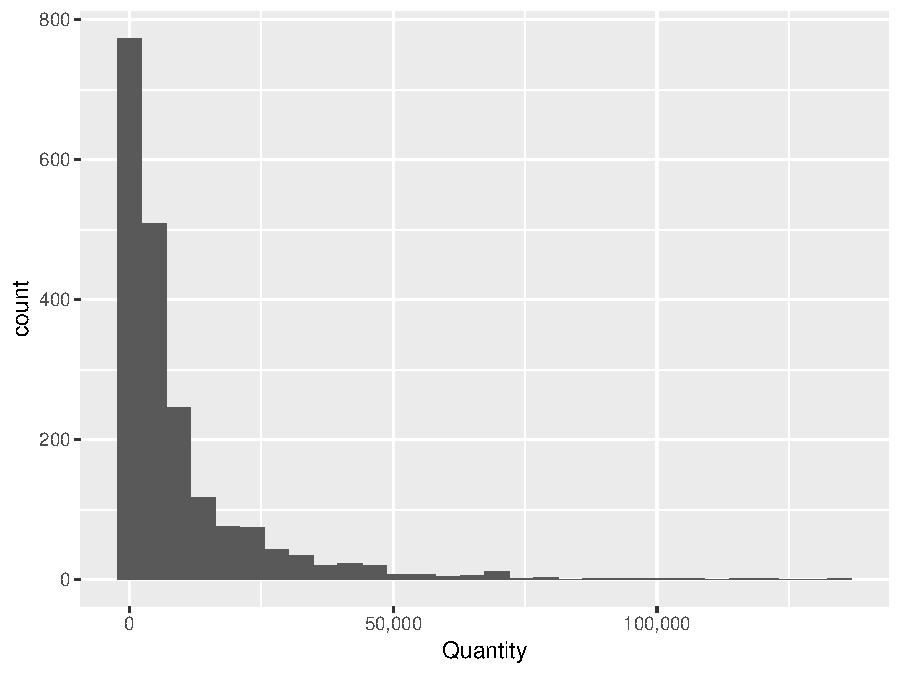
\includegraphics{UChicago-MScA-Capstone_files/figure-latex/Quantity_Histogram-1.pdf}
\caption{(\#fig:Quantity\_Histogram)Histogram of Quantity}
\end{figure}
Figure .

\section*{Modeling results}\label{modeling-results}
\addcontentsline{toc}{section}{Modeling results}

First, use a \texttt{t.test()} to test \emph{if} dosage leads to growth
of incisor length. From the results below, it appears every test rejects
the null hypothesis.
\begin{Shaded}
\begin{Highlighting}[]
\CommentTok{#kable(testAgg, digit = 7, align = "r", caption = "t-test results", }
\CommentTok{#      format = "latex", longtable = TRUE)}
\end{Highlighting}
\end{Shaded}
Table \ref{tab:t-test}

\section*{Results of model performance and
validation}\label{results-of-model-performance-and-validation}
\addcontentsline{toc}{section}{Results of model performance and
validation}

Next, subset the \texttt{ToothGrowth} data into seperate data sets
defined by supplement dose of 0.5, 1, and 2 mg. This allow us to
controlling for dose increases of \emph{economic} significance.

Subset tooth data into a separate \texttt{data.frame} for each dosage
level. Then Execute the \texttt{t.test()} function for the dosage of 0.5
mg and display the results.

\chapter*{Conclusion}\label{conclusion}
\addcontentsline{toc}{chapter}{Conclusion}

This section includes a concise summary of the findings. Your summary
might be organized by the research objectives or hypotheses. Make sure
you address the extent to which research objectives are achieved, and if
they are not achieved, explain why. Make sure to interpret your findings
in a way that acknowledges the limitations of the research. That is, do
not extrapolate the insights derived from your research to situations
you have not examined.

\emph{While increasing dosage leads to larger incisor length, the choice
of delivery mechanism between Orange Juice and Vitamin C does not seem
to make a difference. However, at very low levels, Orange Juice appears
more effective, displaying higher average growth.}

\chapter*{Recommendations}\label{recommendations}
\addcontentsline{toc}{chapter}{Recommendations}

Includes guidelines as to ways in which your results should or could be
used in practice. You may discuss other uses of your results, if there
are any. The ways to extend your analysis and the benefits of doing so
might be included in this section as well.

\appendix

\chapter{The First Appendix}\label{the-first-appendix}

This first appendix includes all of the R chunks of code that were
hidden throughout the document (using the \texttt{include\ =\ FALSE}
chunk tag) to help with readibility and/or setup.

\textbf{In section} \ref{pressure-plot}:

\textbf{In section \ref{ref-labels}:}

\chapter{A Second Appendix, for
example}\label{a-second-appendix-for-example}

\chapter*{References}\label{references}
\addcontentsline{toc}{chapter}{References}

Placeholder


% Index?

\end{document}
